\begin{figure}[tbp]
\begin{center}
\includegraphics[width=0.48\textwidth]{Cl_rsd_sn_z1z2.eps}
\end{center}
\vspace{-0.7cm}
\caption{(Top) Relative strength of kSZ signal, within a box of $\Delta \chi=1200 Mpc/h$. 
    (Bottom) predicted S/N, assuming Planck noise, $\Delta \ell/\ell=0.1$, $f_{sky}=0.8$. 
}
\label{fig:sn}
\end{figure}
%In real surveys, when we calculate the cross angular power spectrum $C_l$ between reconstructed kSZ signals and CMB measurements, we will have to face statistical errors. 
%They can be approximated as:
We use the statistical error to estimate the S/N ratio for real surveys, 
taking into account the contamination from primary CMB and facility noises.
%\begin{eqnarray}
 %   \frac{\Delta C_l}{C_l}\simeq \frac{1}{r\sqrt{(2l+1)\Delta l f_{sky}}}\sqrt{\frac{C_l^{\mr{CMB}}+C_l^{kSZ}+C_l^{\mr{CMB},N}}{C_l^{kSZ,\Delta z}}(1+\frac{C^N_{\hat \Theta}}{C_{\hat \Theta}})}\,
%\end{eqnarray}
\begin{eqnarray}
    \frac{S}{N}&=&\frac{C_l}{\Delta C_l}\\\nonumber
               &\simeq&
    r\sqrt{(2\ell+1)\Delta l f_\mathrm{sky}}\sqrt{\frac{C_l^{\mathrm{kSZ},\Delta z}}{C_l^{\mr{CMB}}+C_l^\mathrm{kSZ}+C_l^{\mr{CMB},N}}}
\end{eqnarray}
Where $C_l^\mathrm{CMB}$ is the angular powerspectrum of primary CMB; 
$C_l^\mathrm{CMB,N}$ indicates the facility noises; 
$C_l^{\mathrm{kSZ},\Delta z}$ is the kSZ signal from a certain redshift bin; 
r is the correlation coefficients we get; 
$f_\mathrm{sky}$ is the percent of sky area covered by both surveys.

In our case, we calculate $C_l^\mr{CMB}$ from CAMB \cite{CAMB}. 
We use Planck 2015 results \cite{Planck2015} at 217GHz to estimate $C_l^\mr{CMB,N}$.
$C_l^\mathrm{CMB,N}=(\sigma_{p,T}\theta_\mathrm{FWHM})^2W_l^{-2}$;  
where $\sigma_{p,T}=8.7\mu K_\mathrm{CMB}$ is Sensitivity per beam solid angle, 
$\theta_\mathrm{FWHM}\sim 5'$ is the effective beam FWHM, 
$W_l=\exp[-\ell(\ell+1)/2\ell^2_\mathrm{beam}]$ is the smoothing window function, 
with $\ell _\mathrm{beam}=\sqrt{8\ln2}/\theta_\mathrm{FWHM}$. 
We choose $f_\mathrm{sky}=0.8$, since it is feasible for 21 cm intensity mapping to survey large sky areas. 
We choose $\Delta \ell/\ell=0.1$. 
And for $C_l^{\mathrm{kSZ},\Delta z}$, we choose two bins of size 1200 Mpc/h, centered at redshift 1,2 respectively.

In Fig.\ref{fig:sn}, we plot the S/N level for the two redshift bins. 
The S/N will exceeds 3 from $\ell \sim 500-3000$. 
The overall S/N for $z=1$ is 45, and for $z=2$ is 59. 

Since we only use the correlation calculated from tidal reconstructed field, the S/N shall be higher for $z=2$  
combining tidal reconstructed field and foreground filtered field. 
%Moreover, since $C_l^{kSZ}$ is relatively flat, 
%it is possible to bin it into larger $\Delta l$. 
%eg. \cite{Hill16} choose $\Delta l=200$, and this will yield better S/N for $\ell <2000$ in Fig.\ref{fig:sn}.

%What's more, Planck's noise level is far from ideal. If we consider the case of $4_\mathrm{th}$ generation facilities, there will also be a giant leap for S/N at large l, 
%assuming clean substraction of CMB lensing. 
